% Overizcht feest:
% Datum \$DATUMFEEST
% Aantal gasten \$GROEPGROTE
% Waarvan kinderen \$KINDEREN
% Betreft: \$BETREFT
% Begintijd: \$BEGINTIJD
% \$STARTPLANNING

\documentclass{scrartcl}
\usepackage[dutch]{babel}
\usepackage{fancyhdr}
\usepackage{wallpaper}
\usepackage[official]{eurosym}
\usepackage{background}
\usepackage{url}

\graphicspath{{img/}}

\backgroundsetup{
  scale=1,
  color=black,
  opacity=1,
  angle=0,
  position=current page.south,
  vshift=90pt,
  contents={%
  \small\sffamily%
  \begin{minipage}{.8\textwidth}
	\center
	\large Restaurant De Huiskamer \\
	\tiny Kerkdijk 2 - $7964KB$ Ansen - tel 0522-471280 - KvK 04005343 -  info@dehuiskamer.com \\
	IBAN NL07 SNSB 095.65.49.721 - BTW nr: 8094.43867B01 \\
	\url{www.dehuiskamer.com} - \url{www.de2dekamer.nl} - \url{m.facebook.com/RestaurantDeHuiskamer}
  \end{minipage}\hspace{.02\textwidth}%
  \begin{minipage}{.18\textwidth}
	  \raggedleft
  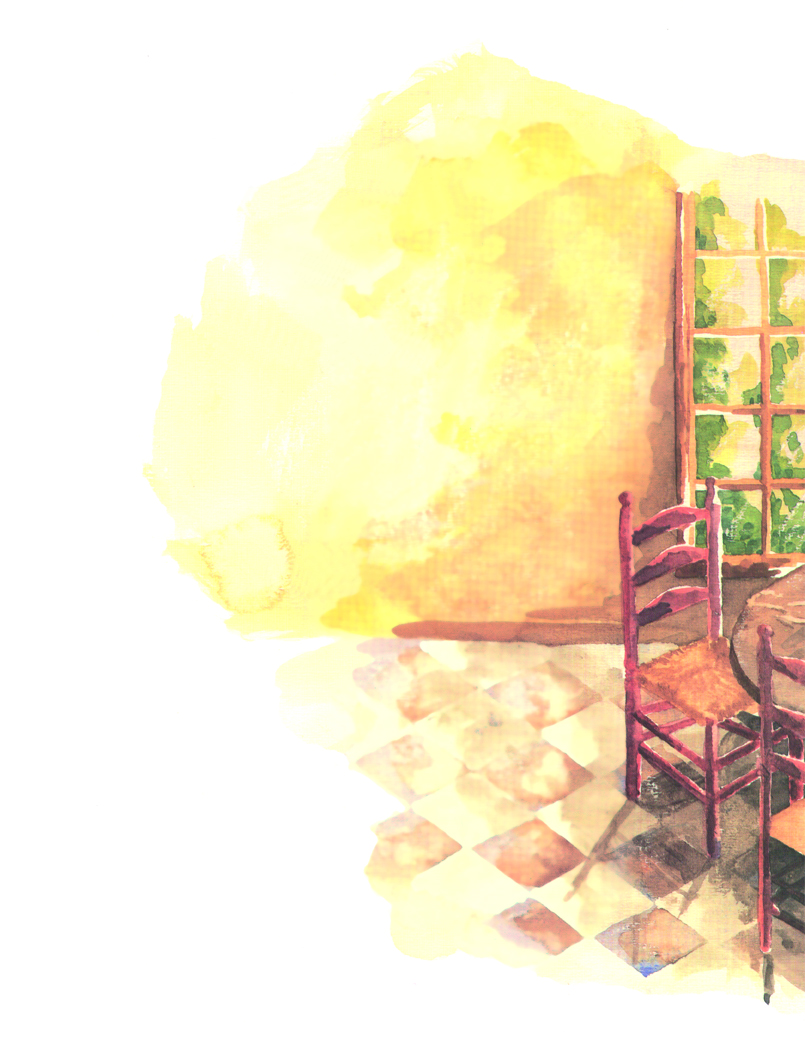
\includegraphics[width=\linewidth,height=70pt,keepaspectratio]{logo2kleur}
  \end{minipage}%
  }
}

\pagestyle{empty}
\renewcommand\headrulewidth{0pt}
\chead{\large Restaurant De Huiskamer \\
\small Ansen $\quad$ tel $0522-471280$}
\begin{document}
\ThisURCornerWallPaper{0.25}{img/logo.jpg}

\title{Restaurant De Huiskamer}
\date{Ansen, \today}
\maketitle
\thispagestyle{empty}

\begin{flushright}
	\$NAAM \\
	\$ADRESS \\
	\$POSTCODE \$PLAATS
\end{flushright}
\section*{Betreft: offerte}
\begin{tabular}{l r}
  E-mail & \$EMAIL  \\
  Tel & \$TEL  \\
\end{tabular}

\subsubsection*{Geachte \$NAAM,}

Naar aanleiding van ons gesprek ontvangt u hierbij een vrijblijvende offerte
voor een \$BETREFT op \$DATUMFEEST

Uitgaande van \$GROEPGROTE gasten en \$KINDEREN kinderen kan dit er als volgt uit zien:

\$DRAAIBOEK

\newpage

\subsection*{Kosten specificatie}
Uigaande van \$GROEPGROTE gasten en \$KINDEREN kinderen.

\$PRIJSOVERZICHT

\subsection*{Bijzonderheden}

\$BIJZONDERHEDEN

\$EXTRAPUNTEN

We hopen uw wensen op de juiste wijze te hebben vertaald, in afwachting op uw reactie,

Met gastvije groet,

Pedro Klooster

\newpage

\section*{Activiteit details}

\$ACTIVITEITDETAILS

\section*{Dieet}

\$DIEET

\end{document}
